\documentclass[11pt,a4paper]{book}

\usepackage[utf8]{inputenc}
\usepackage{amsmath, amssymb, amsthm}
\usepackage{graphicx}
\usepackage{float}
\usepackage{amsthm}
\usepackage{geometry}
\usepackage{tikz}
\usepackage{pgfplots}
\usepackage{caption}
\pgfplotsset{compat=1.18}


\geometry{a4paper, total={171mm,257mm}, left=20mm, top=20mm}
\title{My Exercise Solution to Apostol's Calculus}
\author{songyuncen}
\date{2024.12.26}

\theoremstyle{definition}
\newtheorem{exercise}{Exercise}
\newtheorem{solution}{Solution}

\begin{document}
\maketitle
\chapter*{I. INTRODUCTION}
\addcontentsline{toc}{chapter}{INTRODUCTION}
\section*{Part 1. Historical Introduction}
\subsection*{I 1.4 Exercises}

% 1 

\begin{exercise}
  \textbf{(a)} Modify the region in Figure I.3 by assuming that the ordinate at each $x$  is $2x^2$ instead of $x^2$.
  Draw the new figure. Check through the principal steps in the foregoing section and 
  find what effect this has on the calculation of the area. Do the same if the ordinate
  at each $x$ is \textbf{(b)} $3x^2$, \textbf{(c)} $\frac{1}{4}x^2$, \textbf{(d)} $2x^2 + 1$, \textbf{(e)} $ax^2 + c$.
\end{exercise}

\begin{solution}{\ \\}
  \textbf{(a)}
  % draw
  \begin{figure}[H]
    \centering
    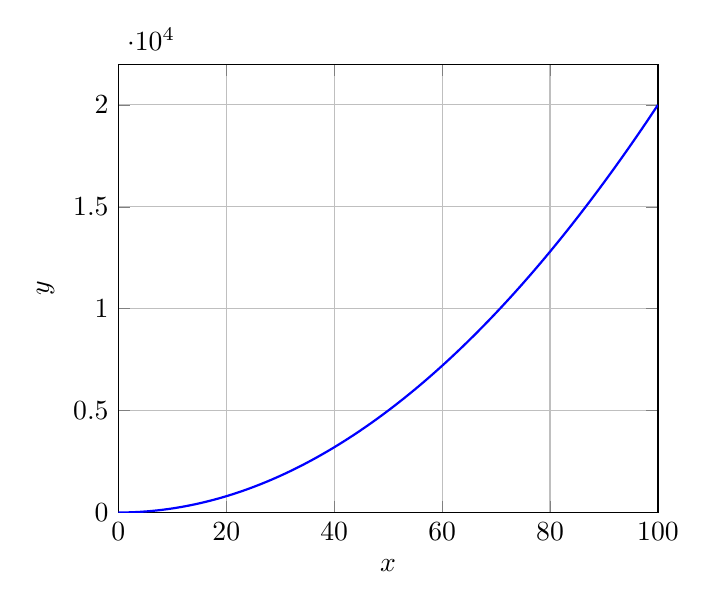
\begin{tikzpicture}
      \begin{axis}[
          xlabel=$x$,
          ylabel=$y$,
          xmin=0,
          xmax=100,
          ymin=0,
          domain=0:100,
          samples=100,
          smooth,
          no markers,
          grid=major
        ]
        \addplot[thick, blue] {2*x^2};
      \end{axis}
    \end{tikzpicture}
    \caption*{Graph of $f(x)=2x^2$ from 0 to 100}
  \end{figure}
  % caculation
  The sum of the areas of all the outer rectangles is
  \[
  S_n = \frac{2b^3}{n^3} \left( 1^2 + 2^2 + \cdots + n^2 \right) 
  \]
  and the sum of the areas of all the inner rectangles is
  \[
  s_n = \frac{2b^3}{n^3} \left( 1^2 + 2^2 + \cdots + (n-1)^2 \right)
  \].

  From identity
  \[
  \tag{I.3} 1^2 + 2^2 + \cdots + n^2 = \frac{n^3}{3} + \frac{n^2}{2} + \frac{n}{6}
  \]
  we have the inequalities
  \[
  \tag{I.5} 1^2 + 2^2 + \cdots + (n-1)^2 < \frac{n^3}{3} < 1^2 + 2^2 + \cdots + n^2.
  \]

  
  If we multiply both sides of (I.5) by $2b^3/n^3$ and make use of the equations of sum of areas, we get
  \[
  s_n < \frac{2b^3}{3} < S_n \tag{1}
  \]
  for every $n$. We already know the area $A$ of the graph is between $s_n$ and $S_n$, so if we can 
  show that $2b^3/3$ is the only number which lies between $s_n$ and $S_n$ for every $n$, we can conclude that $A = 2b^3/3$.

  There are only three conditions for a number $B$ which satisfied $s_n < B < S_n$: $B > 2b^3/3$, $B < 2b^3/3$, and $B = 2b^3/3$.

  If $B > 2b^3/3$, we add $\frac{2b^3}{n^3}n^2$ to left side and middle side of (1) to get
  \[
  s_n + \frac{2b^3}{n^3}n^2 < \frac{2b^3}{3} + \frac{2b^3}{n^3}n^2
  \]
  which is equivalent to
  \[
  B < S_n < \frac{2b^3}{3} + \frac{2b^3}{n}.
  \]
  Since $B - 2b^3/3 > 0$, we get
  \[
  n < \frac{2b^3}{B - 2b^3/3}.
  \]
  for every integr $n \ge 1$. This is impossible, so $B > 2b^3/3$ is false.

  If $B < 2b^3/3$, we substract $\frac{2b^3}{n^3}n^2$ from right side and middle side of (1) to get
  \[
  \frac{2b^3}{3} - \frac{2b^3}{n^3}n^2 < Sn - \frac{2b^3}{n^3}n^2
  \]
  which is equivalent to
  \[
  \frac{2b^3}{3} - \frac{2b^3}{n} < s_n < B.
  \]
  Since $2b^3/3 - B > 0$, we get
  \[
  n < \frac{2b^3}{2b^3/3 - B}.
  \]
  for every integr $n \ge 1$. This is impossible, so $B < 2b^3/3$ is false.

  Therefore, $2b^3/3$ is the only number which lies between $s_n$ and $S_n$ for every $n$.

  \vspace{2\baselineskip}
  \textbf{(b), (c)} The results are similar to (a). The area of the graph is $b^3$ and $\frac{b^3}{12}$ respectively.

  \vspace{2\baselineskip}
  \textbf{(d)} The area of one outer rectangle is
  \[
  \left( \frac{b}{n} \right) \left( 2 \left( \frac{kb}{n} \right)^2 + 1 \right) = \frac{2b^3}{n^3}k^2 + \frac{b}{n}
  \]

  The sum of the areas of all the outer rectangles is
  \[
    S_n = \frac{2b^3}{n^3} \left( 1^2 + 2^2 + \cdots + n^2 \right) + b.
  \]

  The sum of the areas of all the inner rectangles is
  \[
    s_n = \frac{2b^3}{n^3} \left( 1^2 + 2^2 + \cdots + (n-1)^2 \right) + \frac{(n-1)b}{n}.
  \]

  From inequalities (I.5) we have
  \[
  \frac{2b^3}{n^3} \left(1^2 + 2^2 + \cdots + (n-1)^2 \right) < \frac{2b^3}{3} < \frac{2b^3}{n^3} \left( 1^2 + 2^2 + \cdots + n^2 \right).
  \]
  Add $b$ to both sides of the inequality, we get
  \[
  s_n < \frac{2b^3}{n^3}\left( 1^2 + 2^2 + \cdots + (n-1)^2 \right) + b < \frac{2b^3}{3} + b < S_n.
  \]
  Which is equivalent to
  \[
  s_n < \frac{2b^3}{3} + b < S_n. \tag{2}
  \]

  for every $n \ge 1$. We already know the area $A$ of the graph is between $s_n$ and $S_n$, so if we can 
  show that $2b^3/3 + b$ is the only number which lies between $s_n$ and $S_n$ for every $n$, we can conclude that $A = 2b^3/3 + b$.

  There are only three conditions for a number $B$ which satisfied $s_n < B < S_n$: $B > 2b^3/3 + b$, $B < 2b^3/3 + b$, and $B = 2b^3/3 + b$.

  If $B > 2b^3/3 + b$, we add $\frac{2b^3}{n^3}n^2 + \frac{b}{n}$ to left side and middle side of (2) to get
  \[
  s_n + \frac{2b^3}{n^3}n^2 + \frac{b}{n} < \frac{2b^3}{3} + b + \frac{2b^3}{n^3}n^2 + \frac{b}{n}
  \]
  which is equivalent to
  \[
  B < S_n < \frac{2b^3}{3} + b + \frac{2b^3 + b}{n}.
  \]
  Since $B - 2b^3/3 - b > 0$, we get
  \[
  n < \frac{2b^3 + b}{B - 2b^3/3 - b}.
  \]
  for every integr $n \ge 1$. This is impossible, so $B > 2b^3/3 + b$ is false.

  If $B < 2b^3/3 + b$, we substract $\frac{2b^3}{n^3}n^2 + \frac{b}{n}$ from right side and middle side of (2) to get
  \[
  \frac{2b^3}{3} + b - \frac{2b^3}{n^3}n^2 - \frac{b}{n} < Sn - \frac{2b^3}{n^3}n^2 - \frac{b}{n}
  \]
  which is equivalent to
  \[
  \frac{2b^3}{3} + b - \frac{2b^3}{n} - \frac{b}{n} < s_n < B.
  \]
  Since $2b^3/3 + b - B > 0$, we get
  \[
  n < \frac{2b^3 + b}{2b^3/3 + b - B}.
  \]
  for every integr $n \ge 1$. This is impossible, so $B < 2b^3/3 + b$ is false.

  Therefore, $2b^3/3 + b$ is the only number which lies between $s_n$ and $S_n$ for every $n$.

  \vspace{2\baselineskip}
  \textbf{(e)} The result are similar to (d). The area of the graph is $ab^3 + cb$.
\end{solution}

% 2

\begin{exercise}\label{ex:2}
  Modify the region in Figure I.3 by assuming that the ordinate at each $x$ is $x^3$ instead of $x^2$.
  Draw the new figure.

  (a) Use a construction similar to that iluustrated in Figure I.5 and show that the outer and inner
  sums $S_n$ and $s_n$ are given by
  \[
  S_n = \frac{b^4}{n^4} \left( 1^3 + 2^3 + \cdots + n^3 \right), \quad s_n = \frac{b^4}{n^4} \left( 1^3 + 2^3 + \cdots + (n-1)^3 \right).
  \]

  (b) Use the inequalities (which can be proved by mathematical induction; see Section I4.2)
  \[
  \tag{I.12} 1^3 + 2^3 + \cdots + (n - 1)^3 < \frac{n^4}{4} < 1^3 + 2^3 + \cdots + n^3
  \]
  to show that $s_n < b^4 /4 < S_n$ for every $n$, and prove that $b^4/4$ is the only number which lies between $s_n$ and $S_n$ for every $n$.

  (c) What number takes the place of $b^4/4$ if the ordinate at each $x$ is $ax^3+c$?
\end{exercise}

\begin{solution}
  \textbf{(a)}
    % draw
    \begin{figure}[H]
      \centering
      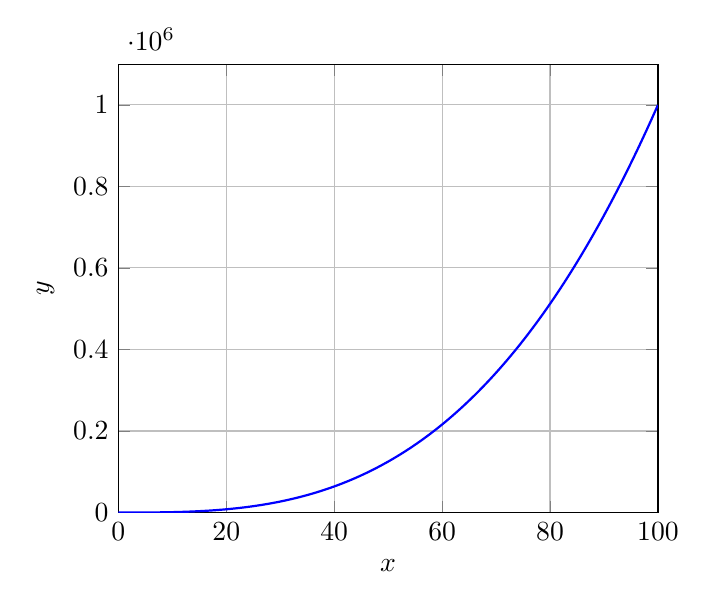
\begin{tikzpicture}
        \begin{axis}[
            xlabel=$x$,
            ylabel=$y$,
            xmin=0,
            xmax=100,
            ymin=0,
            domain=0:100,
            samples=100,
            smooth,
            no markers,
            grid=major
          ]
          \addplot[thick, blue] {x^3};
        \end{axis}
      \end{tikzpicture}
      \caption*{Graph of $f(x)=x^3$ from 0 to 100}
    \end{figure}

  \vspace{2\baselineskip}
  \textbf{(b)}
  Multiply the both side of inequalities (I.12) by $b^4/n^4$ and we get
  \[
  s_n < \frac{b^4}{4} < S_n
  \]
  for every $n$. We already know the area $A$ of the graph is between $s_n$ and $S_n$, so if we can
  show that $b^4/4$ is the only number which lies between $s_n$ and $S_n$ for every $n$, we can conclude that $A = b^4/4$.

  There are only three conditions for a number $B$ which satisfied $s_n < B < S_n$: $B > b^4/4$, $B < b^4/4$, and $B = b^4/4$.

  If $B > b^4/4$, we add $\frac{b^4}{n^4}n^3$ to left side and middle side of the inequality (I.12) to get
  \[
  B < S_n < \frac{b^4}{4} + \frac{b^4}{n}.
  \]
  Since $B - b^4/4 > 0$, we get
  \[
  n < \frac{b^4}{B - b^4/4}
  \]
  for every integr $n \ge 1$. This is impossible, so $B > b^4/4$ is false.

  If $B < b^4/4$, we substract $\frac{b^4}{n^4}n^3$ from right side and middle side of the inequality (I.12) to get
  \[
  \frac{b^4}{4} - \frac{b^4}{n^4}n^3 < S_n - \frac{b^4}{n^4}n^3 = s_n < B.
  \]
  Since $b^4/4 - B > 0$, we get
  \[
  n < \frac{b^4}{b^4/4 - B}
  \]
  for every integr $n \ge 1$. This is impossible, so $B < b^4/4$ is false.

  Therefore, $b^4/4$ is the only number which lies between $s_n$ and $S_n$ for every $n$.

  \vspace{2\baselineskip}
  \textbf{(c)}
  The problem is similar to Exercise \ref{ex:2}.(e), and the result is
  \[
  \frac{ab^4}{4} + cb.
  \]
\end{solution}

% 3 

\begin{exercise}
  The inequalities (I.5) and (I.12) are special cases of the more general inequalities
  \[
  \tag{I.13}  1^k + 2^k + \cdot + (n - 1)^k < \frac{n^{k+1}}{k+1} < 1^k + 2^k + \cdot + n^k
  \]
  that are vaild for every integer $n \ge 1$ and every integer $k \ge 1$. Assume the validity of (I.13) and generalize the results of Exercise \ref{ex:1}
\end{exercise}

\begin{solution}
  The more genreal result of Exercise \ref{ex:2} is that: the area below the region of 
  graph specified by $ax^k + c$ between the interval of $0$ and $b$ is 
  \[
  \frac{ab^{k+1}}{k+1} + bc.
  \]
\end{solution}

\end{document}
